\newpage
\section{Specyfika projektów informatycznych}
Skuteczne dostarczanie oczekiwanych korzyści z projektów informatycznych stanowi wyzwanie dla wielu organizacji. \autocite{robey} Badania branżowe \autocite{rubinstein} oraz raporty rządowe \autocite{canada}\autocite{gov} wskazują na konieczność poprawy efektywności realizacji projektów IT. Połączenie rosnącej zależności od systemów informatycznych oraz wzrastających kosztów wdrażania takich projektów sugeruje, że wydajność projektów IT jest kluczową kwestią organizacyjną. \autocite{ryzyka}

Jednak specyficzna natura projektów informatycznych sprawia, że są one szczególnie wymagające. Projekty IT charakteryzują się wyjątkową różnorodnością w porównaniu z inicjatywami w innych branżach. Niektóre projekty ograniczają się do wdrażania gotowych rozwiązań sprzętowych i oprogramowania przez małe grupy specjalistów. Inne wymagają zaangażowania setek osób w analizę procesów biznesowych wielu podmiotów oraz współtworzenie dopasowanych systemów informatycznych. Ważnym aspektem projektów IT jest różnorodność dostępnych technologii. Nawet w prostych projektach sprzętowych występuje szerokie spektrum urządzeń – od komputerów stacjonarnych po infrastrukturę sieciową, terminale mobilne czy urządzenia IoT. Łączność w takich projektach może opierać się na technologiach bezprzewodowych, światłowodowych, komórkowych lub satelitarnych. Złożoność ta jest jednak niewielka w porównaniu do projektów programistycznych, gdzie ilość dostępnych rozwiązań i technologii jest znacznie większa.

Projekty informatyczne obejmują praktycznie wszystkie dziedziny gospodarki i funkcje biznesowe. Kompetencje niezbędne do zarządzania projektem IT dla studia animacji różnią się od tych wymaganych przy modernizacji rządowego systemu podatkowego czy wdrażaniu nowej sieci telekomunikacyjnej. Ta różnorodność, połączona z dynamicznym rozwojem branży i mnogością technologii, powoduje, że projekty IT znacząco wyróżniają się na tle innych dziedzin. \autocite{ITPM}

\subsection{Niechęć do projektów informatycznych}
Kwestia projektowania i wdrażania systemów informatycznych bywa często postrzegana jako abstrakcyjna, nawet przez osoby regularnie korzystające z technologii w życiu zawodowym i prywatnym. Użytkownicy nie zawsze zdają sobie sprawę z powiązań między tym, co widzą na ekranie, a złożonym procesem tworzenia oprogramowania. Problem ten sięga głębiej – często pomija się zależność między funkcjonalnością systemu a koniecznością przeprowadzenia rzetelnego projektu w celu jej wprowadzenia. Próby zaangażowania przyszłych użytkowników w definiowanie wymagań spotykają się z oporem, gdyż w społecznym odbiorze wystarczające wydaje się wykorzystanie już istniejących narzędzi. W przypadku skomplikowanych projektów innowacyjnych ujawnia się stereotypowe przekonanie, że proces adaptacji technologii w organizacji jest uciążliwy i zakłóca codzienne obowiązki.

Mimo powszechnego korzystania z oprogramowania, obserwuje się niedostatek wiedzy o wzajemnych powiązaniach poszczególnych etapów tworzenia systemów oraz ich ciągłej ewolucji. W ostatnich latach nastąpiła jednak znacząca zmiana. Współczesne podejście do wytwarzania oprogramowania kładzie nacisk na dostosowanie rozwiązań do realnych potrzeb użytkowników końcowych oraz zwiększenie efektywności ekonomicznej projektów. Ta orientacja kontrastuje z bezrefleksyjną implementacją technologii za wszelką cenę z początku stulecia i stanowi istotny postęp. \autocite{ITPMChmielarz}

Thomas i Hunt w swojej książce zawarli ważne zdanie na ten temat: "Programiści pomagają użytkownikom zrozumieć, czego użytkownicy chcą". \autocite{pragmatic} To stwierdzenie uwypukla kluczową rolę zrozumienia i realizacji potrzeb użytkowników w projektach informatycznych.

Możemy zbudować system, który jest sukcesem technicznym, lecz porażką organizacyjną. Systemy informatyczne – produkty projektów IT – są planowaną zmianą organizacyjną. Technologia informatyczna jest czynnikiem umożliwiającym tworzenie nowych produktów, usług i procesów, które mogą zmieniać istniejące relacje między organizacją a jej klientami lub dostawcami, a także między osobami w ramach samej organizacji.  

Ta zmiana może stanowić zagrożenie dla wielu grup. Dlatego ludzie mogą nie zawsze być przychylni nowemu systemowi informatycznemu – niezależnie od tego, jak dobrze został zbudowany lub jak nowoczesne są zastosowane technologie, narzędzia i techniki. Z drugiej strony, osoby w organizacji mogą słusznie opierać się systemowi, który nie działa prawidłowo lub nie spełnia ich oczekiwań. \autocite{ITPMMarchewka}

Opisane wyzwania dotyczą niestety także części specjalistów IT, którzy niekiedy ograniczają się do stosowania sprawdzonych, lecz nie zawsze adekwatnych schematów. Przekonanie, że „w informatyce nie ma już nic nowego” czy „wszystkie innowacje zostały wdrożone” bywa pułapką utrudniającą odpowiedź na zmieniającą się rzeczywistość – zarówno wirtualną, jak i realną. \autocite{ITPMChmielarz}

Konieczne jest podejście, które nie stawia strony technicznej ponad organizacyjną ani odwrotnie. Aby dostarczyć udany projekt, należy zachować równowagę między aspektami technicznymi a organizacyjnymi projektów IT. \autocite{ITPMMarchewka}

\subsection{Cykl życia w projektach informatycznych}
W inżynierii oprogramowania wyróżnia się różne rodzaje projektów (np. rozwój produktu, usługi outsourcingowe, konserwacja oprogramowania, tworzenie usług itp.). W cyklu życia produktu programistycznego może być wymaganych wiele projektów. Przykładowo, na etapie koncepcji produktu może zostać przeprowadzony projekt w celu określenia potrzeb klientów i wymagań rynkowych lub podczas konserwacji może zostać zrealizowany projekt mający na celu opracowanie kolejnej wersji produktu. \autocite{swebok}

\subsubsection{Cykl życia projektu}
Podobnie jak wszystkie żywe istoty, projekty mają cykle życia, w których rodzą się, rosną, osiągają szczyt, upadają, a następnie kończą się. \autocite{gido} Chociaż cykle życia projektów mogą się różnić w zależności od branży lub projektu, wszystkie cykle życia projektów będą miały początek, środek i koniec. \autocite{Rosenau} Cykl życia projektu (PLC) jest to ciąg faz, przez które projekt przechodzi od rozpoczęcia po zakończenie. \autocite{pmbok7} Faza projektu zaś to zbiór logicznie powiązanych działań, które kończą się wytworzeniem jednego lub więcej rezultatów (np. dokumentacji, prototypu, gotowego modułu). Każda faza ma określone ramy czasowe – rozpoczyna się i kończy w punkcie kontrolnym (ang. phase gate). Według PMBOK® Guide, podstawowy cykl obejmuje cztery etapy:
\begin{itemize}
    \item rozpoczęcie projektu,
    \item organizacja i przygotowanie,
    \item realizacja prac,
    \item zakończenie projektu.
\end{itemize}

Ogólnie rzecz biorąc, cykle życia projektu określają, jaka praca zostanie wykonana w każdej fazie, jakie produkty zostaną wyprodukowane i kiedy, kto jest zaangażowany w każdą fazę oraz w jaki sposób kierownictwo będzie kontrolować i zatwierdzać pracę wyprodukowaną w każdej fazie. Produktem może być faktycznie jakiś produkt lub usługa, taka jak na przykład raport techniczny czy sesja szkoleniowa. \autocite{ITPM}

\subsubsection{Cykl życia produktu}
Podobnie jak projekty, produkty również mają swój cykl życia. Cykl życia produktu to seria faz, które reprezentują ewolucję produktu, od koncepcji, poprzez dostawę, wzrost, dojrzałość, aż do wycofania. \autocite{pmbok6}

Ta definicja nie jest specyficzna dla systemów programistycznych, lecz ma zastosowanie ogólnie do wszystkich produktów. Podobnie koncepcja cyklu życia, powiązana z pojęciem produktu, nie jest wyłączną domeną inżynierii oprogramowania.

Systemy programistyczne zawierają jednostki oprogramowania (ang. software units), które są „podstawowymi komponentami architektury oprogramowania, podlegającymi niezależnemu testowaniu”. Cykl życia systemu programistycznego (uwzględniający interdyscyplinarne podejście inżynierii oprogramowania) obejmuje wszystkie procesy, działania i zadania – od powstania koncepcji systemu aż do jego wycofania, włączając w to produkcję, eksploatację, ewolucję, a także – w razie potrzeby – pozyskanie i dostarczenie. Analogicznie można rozpatrywać cykl życia pojedynczego elementu systemu (np. jednostki oprogramowania). \autocite{swebok}

Większość specjalistów IT zna koncepcję cyklu życia produktu, szczególnie w przypadku rozwoju oprogramowania. \autocite{ITPM} Choć projekty podlegają cyklowi życia projektu (PLC), rozwój systemów informatycznych podlega cyklowi życia produktu. Najpopularniejszym cyklem w branży IT jest Cykl Życia Oprogramowania (SDLC), który obejmuje sekwencyjne fazy, przez które przechodzi system informatyczny w trakcie swojego istnienia. \autocite{ITPMMarchewka} SDLC określa logiczną kolejność etapów rozwoju systemu oraz decyduje o przejściu od jednej czynności do kolejnej. \autocite{McConnell}

Podstawowe fazy SDLC to:
\begin{itemize}
    \item planowanie,
    \item analiza,
    \item projektowanie,
    \item wdrożenie,
    \item utrzymanie i wsparcie. \autocite{ITPMMarchewka}
\end{itemize}

\subsubsection{Integracja PLC i SDLC w projektach informatycznych}
Kluczowa różnica między cyklem życia projektu a cyklem życia oprogramowania polega na tym, że PLC koncentruje się na zarządzaniu procesem realizacji projektu, podczas gdy SDLC dotyczy tworzenia i implementacji produktu – systemu informatycznego. W projektach IT oba cykle często się przenikają – np. fazy SDLC (projektowanie) realizowane są w ramach etapów PLC. Połączenie zarządzania projektem z cyklem życia oprogramowania jest cechą charakterystyczną projektów IT. Jak pokazuje Rysunek 4.1, SDLC stanowi część PLC, ponieważ większość działań związanych z rozwojem systemu odbywa się w fazie realizacji projektu. Etapy zamknięcia i ewaluacji projektu następują dopiero po wdrożeniu systemu. \autocite{ITPMMarchewka}

\begin{figure}
    \centering
    \caption{Porównanie cyklu życia oprogramowania do cyklu życia projektu}
    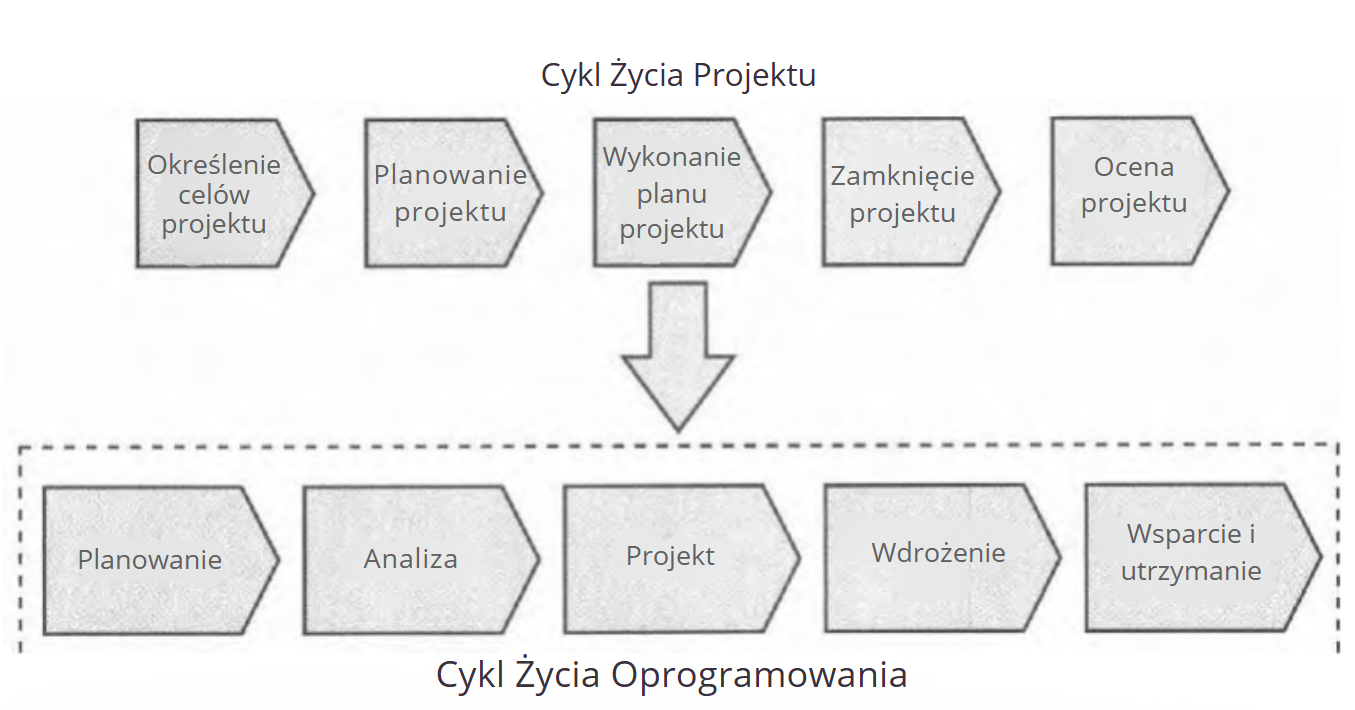
\includegraphics[width=1\linewidth]{img/plc_PL.png}
    \caption*{J. T. Marchewka. Information Technology Project management. Northern Illinois University, 2003}
\end{figure}

\subsection{Modele SDLC}
W inżynierii oprogramowania koncepcja SDLC stanowi podstawę wielu modeli cyklu życia oprogramowania. Modele te tworzą ramy planowania i kontroli procesu tworzenia systemu informatycznego. \autocite{swebok} Wszystkie sugerowane modele SDLC dzielą podstawowe cechy: składają się z sekwencji faz lub kroków, które muszą być przestrzegane i zakończone przez programistów oraz projektantów systemów, aby osiągnąć rozwinięte systemy i dostarczyć wymagane produkty. \autocite{alshamrani2015comparison} Każdy system oprogramowania posiada unikalne cechy odzwierciedlające potrzeby interesariuszy – zarówno biznesowe, jak i techniczne. Odpowiedni cykl życia powinien uwzględniać wszystkie te wymagania. \autocite{swebok} Wybór modelu SDLC powinien być dokonywany na podstawie wymagań projektu. \autocite{arora2016analysis}

PMBOK® krótko opisuje pięć cykli życia produktu lub rozwoju. Dwa czynniki są istotne przy wyborze odpowiedniego cyklu życia: stopień zmienności wymagań oraz częstotliwość dostarczania użytecznych wyników. Na przykład, dla produktu o niskim stopniu zmienności wymagań i niskiej częstotliwości dostarczania, odpowiedni będzie cykl życia predykcyjny. \autocite{pmbok6}\autocite{ITPM}

\begin{itemize}
    \item \textbf{Cykl życia predykcyjny:} Zakres, harmonogram i koszty są określane na wczesnym etapie, a zmiany w zakresie są ściśle kontrolowane. PMI określa również cykle predykcyjne jako model kaskadowy (waterfall). \autocite{pmbok}\autocite{ITPM}
    
    \item \textbf{Cykl życia iteracyjny:} Zakres jest określany na wczesnym etapie, ale szacowania czasu i kosztów są modyfikowane w miarę wzrostu wiedzy zespołu o produkcie. Iteracje służą do rozwijania produktu poprzez powtarzające się cykle, które dodają kolejne funkcjonalności. \autocite{sommerville2015software}\autocite{farley2021}\autocite{pmbok6} Długość iteracji definiuje się dla każdego projektu. \autocite{swebok} To podejście najlepiej sprawdza się w przypadku wysokiego stopnia zmienności i niskiej częstotliwości dostarczania. \autocite{ITPM}
    
    \item \textbf{Cykl życia przyrostowy:} Produkt końcowy jest dostarczany poprzez serię iteracji stopniowo dodających funkcjonalność w określonym przedziale czasowym. Produkt osiąga pełną funkcjonalność dopiero po ostatniej iteracji. \autocite{sommerville2015software}\autocite{farley2021}\autocite{pmbok6} To podejście najlepiej sprawdza się w przypadku niskiego stopnia zmienności i wysokiej częstotliwości dostarczania. \autocite{ITPM}
    
    \item \textbf{Cykl życia adaptacyjny:} Interesariusze definiują i zatwierdzają szczegółowy zakres przed rozpoczęciem iteracji, dostarczając użyteczny produkt na końcu każdej iteracji. PMI określa również cykle adaptacyjne jako zwinne (agile) lub sterowane zmianą. To podejście najlepiej sprawdza się w przypadku wysokiego stopnia zmienności i wysokiej częstotliwości dostarczania. \autocite{pmbok6}\autocite{ITPM}
    
    \item \textbf{Cykl życia hybrydowy:} Jest to kombinacja podejścia adaptacyjnego i predykcyjnego. Oznacza to, że niektóre elementy pochodzą z podejścia predykcyjnego, a inne z podejścia adaptacyjnego. Takie podejście do rozwoju jest przydatne, gdy istnieje niepewność lub ryzyko związane z wymaganiami. Hybrydowe podejście sprawdza się również, gdy dostarczane elementy mogą być modularne lub gdy różne zespoły projektowe mogą opracowywać różne części produktu. Podejście hybrydowe jest bardziej adaptacyjne niż podejście predykcyjne, ale mniej niż podejście w pełni adaptacyjne. \autocite{pmbok7}
\end{itemize}

Kilka modeli cyklu życia stało się dobrze znanych wraz z rozwojem inżynierii oprogramowania od jej początków, dwa z nich zostaną omówione w kolejnych podrozdziałach.

\subsubsection{Model kaskadowy}

Jednym z modeli, który zdobył popularność we wczesnej historii dyscypliny inżynierii oprogramowania, jest model kaskadowy. \autocite{sommerville2015software} Model kaskadowy, zaliczany do modeli predykcyjnych, zakłada określenie zakresu, harmonogramu i kosztów już na wczesnym etapie, a wszelkie zmiany są ściśle kontrolowane. Podejście to obejmuje fazy takie jak: zbieranie wymagań, projekt wstępny, projekt szczegółowy, kodowanie oraz testowanie, przy czym kolejna faza nie może się rozpocząć, dopóki poprzednia nie zostanie zakończona. \autocite{swebok} Po zakończeniu fazy nie wracamy już do niej, dlatego model ten jest zazwyczaj planowany przy użyciu wykresu Gantta. Podstawowe założenie metody kaskadowej polega na zapewnieniu stabilności wymagań. Wymagania określają potrzebne informacje, funkcje, zachowanie, wydajność oraz interfejsy. \autocite{arora2016analysis}

Postęp w modelu kaskadowym przebiega z góry na dół, przypominając wodospad. Model ten wywodzi się z przemysłu produkcyjnego oraz budownictwa, czyli silnie ustrukturyzowanych środowisk fizycznych, w których wprowadzanie zmian po fakcie jest niezwykle kosztowne, a często wręcz niemożliwe. Ponieważ w tamtym czasie nie istniały formalne metodologie tworzenia oprogramowania, ten produkcyjny model został po prostu zaadaptowany do potrzeb rozwoju oprogramowania. \autocite{SDLC}

Pierwszy formalny opis modelu kaskadowego często przypisuje się artykułowi opublikowanemu w 1970 roku przez Winstona W. Royce'a (1929–1995), \autocite{royce1970} chociaż w swoim artykule nie użył on terminu „waterfall” (kaskadowy). Royce przedstawił ten model jako przykład wadliwego, nieskutecznego podejścia. W rzeczywistości właśnie w ten sposób termin ten był najczęściej używany w literaturze dotyczącej inżynierii oprogramowania – jako sposób na krytykę powszechnie stosowanej praktyki wytwarzania oprogramowania. \autocite{SDLC}

Model kaskadowy był jednak użyteczny, gdyż wprowadził systematyzację w rozwoju systemów oprogramowania, czyli inżynierskie podejście do tworzenia produktów programistycznych. \autocite{swebok}

\textbf{Zalety podejścia kaskadowego}
\begin{itemize}
    \item Proste i łatwe w użyciu oraz zrozumieniu.
    \item Fazy nie nakładają się na siebie, co pozwala na efektywne zarządzanie projektem.
    \item Bardzo dobrze sprawdza się w małych projektach.
\end{itemize}

\textbf{Wady podejścia kaskadowego}
\begin{itemize}
    \item Nie można uzyskać akceptacji użytkownika aż do zakończenia całego procesu.
    \item Sukces projektu jest niepewny aż do jego zakończenia.
\end{itemize}

\textbf{Kiedy stosować metodę kaskadową}
\begin{itemize}
    \item Model najlepiej sprawdza się, gdy wszystkie wymagania są jasne, stałe i dobrze określone.
    \item Definicja produktu i wykorzystywana technologia są dobrze znane.
    \item Brak niejednoznacznych wymagań.
    \item Czas trwania projektu jest krótki. \autocite{arora2016analysis}
\end{itemize}

\subsubsection{Agile}

Kolejnym popularnym modelem jest agile. Jest to model iteracyjny, w którym fazy projektu przebiegają równocześnie, tj. równolegle. Wymagania mogą ewoluować na każdym etapie i w każdej fazie. \autocite{arora2016analysis}

Manifest Agile \autocite{agileManifesto} wywołał rewolucję w społeczności inżynierii oprogramowania, wprowadzając przekonanie, że proces powinien być otwarty na zmiany – wymagania mogą być modyfikowane na każdym etapie, jeśli zmienią się potrzeby użytkowników. Kluczowe stały się komunikacja i wzajemne zaufanie między zespołem a klientem. Sygnatariusze Manifestu podkreślali, że choć komunikacja (często twarzą w twarz) i interakcje z klientem są niezwykle istotne, dokumentacja (np. do definiowania wymagań) pozostaje konieczna. Postulowali także małe, przyrostowe dostawy oprogramowania, w przeciwieństwie do modelu kaskadowego, gdzie całość produktu dostarczana jest dopiero na zakończenie projektu. \autocite{swebok}

\begin{figure}
    \centering
    \caption{Wartości Agile}
    
\includegraphics[width=1\linewidth]{img/agile2.png}
    \caption*{Żródło: https://www.intellect.pl/blog/dlaczego-agile/}
\end{figure}

Agile wyraźnie rozróżnia wartości i zasady (np. ciągłe dostarczanie wartości czy zobowiązanie do doskonałości technicznej) od praktyk (takich jak programowanie w parach, planowanie sprintów czy retrospektywy). 
Mentalność Agile, oparta na zasadach takich jak otwartość na zmiany i nacisk na komunikację, różni się od podejścia predykcyjnego, które skupia się na realizacji ustalonych specyfikacji wymagań. Agile pomaga również radzić sobie ze złożonością systemów. \autocite{swebok}

Możemy postrzegać metody zwinne, takie jak Extreme Programming (XP) i Scrum, jako reakcję na modele predykcyjne, które kładą nacisk na "zracjonalizowane, inżynierskie podejście", \autocite{dyba2000} obejmujące szczegółowe planowanie, sformalizowane procesy oraz rygorystyczne wykorzystanie komponentów. \autocite{boehm2002} W przeciwieństwie do nich, metody zwinne odpowiadają na wyzwania nieprzewidywalnego świata, podkreślając wartość, jaką ludzie i ich relacje wnoszą w rozwój oprogramowania. \autocite{dyba2009we}\autocite{nerur2007}

Wokół Agile narosło wiele nieporozumień. Niektórzy myślą, że Agile stanowi kompletną metodę – jednak nie jest ona metodą samą w sobie, lecz zbiorem wartości, zasad i praktyk. Inne błędne przekonanie mówi, że Agile jest szybszy niż model kaskadowy, gdyż nie wymaga tworzenia dokumentacji. Kolejnym mitem jest pogląd, że Agile opiera się na ograniczonym zbiorze metod. 
Mimo rosnącej popularności modelu Agile, skalowanie go na duże projekty i portfele pozostaje wyzwaniem. Obecnie uważa się, że Manifest Agile przyniósł znaczące zmiany, jednak po 20 latach niektórzy autorzy sugerują konieczność aktualizacji pewnych jego zasad. \autocite{swebok}

Agile to nie tylko zbiór technik programistycznych, ale "ruch, ideologia, filozofia". Idąc jeszcze dalej, jeden z twórców Scruma stwierdza: „Agile to emocja”. \autocite{meyer2014agile} Zastosowanie praktyk Agile wykracza poza sam proces inżynierii oprogramowania – terminy takie jak „zwinność biznesowa” oraz „zwinne organizacje” stały się powszechne. Z perspektywy inżynierii oprogramowania Agile umożliwił ponowną inżynierię i lepsze dopasowanie procesów technicznych do strategicznych celów biznesowych. Wykorzystanie podejścia Agile w procesach biznesowych znajduje odzwierciedlenie między innymi w zasadach DevOps oraz w procesach oceny i doskonalenia jakościowych. \autocite{swebok}

\textbf{Zalety podejścia Agile}
\begin{itemize}
    \item Zmiany można wprowadzać bardzo łatwo.
    \item Zmiany można obsłużyć bez dużych kosztów ponownego planowania.
    \item Stałe zaangażowanie zespołu.
\end{itemize}

\textbf{Wady podejścia Agile}
\begin{itemize}
    \item Częściej pojawiają się problemy ze strukturą zespołu niż problemy z planowaniem.
    \item Niepewne terminy planowania.
\end{itemize}

\textbf{Kiedy stosować podejście Agile}
\begin{itemize}
    \item Gdy istnieje ciągła potrzeba wprowadzania zmian.
    \item Gdy zarówno programiści, jak i inni interesariusze mają swobodę sugerowania zmian. \autocite{arora2016analysis}
\end{itemize}

\begin{figure}
    \centering
    \caption{Porównanie modelu kaskadowego z Agile}
    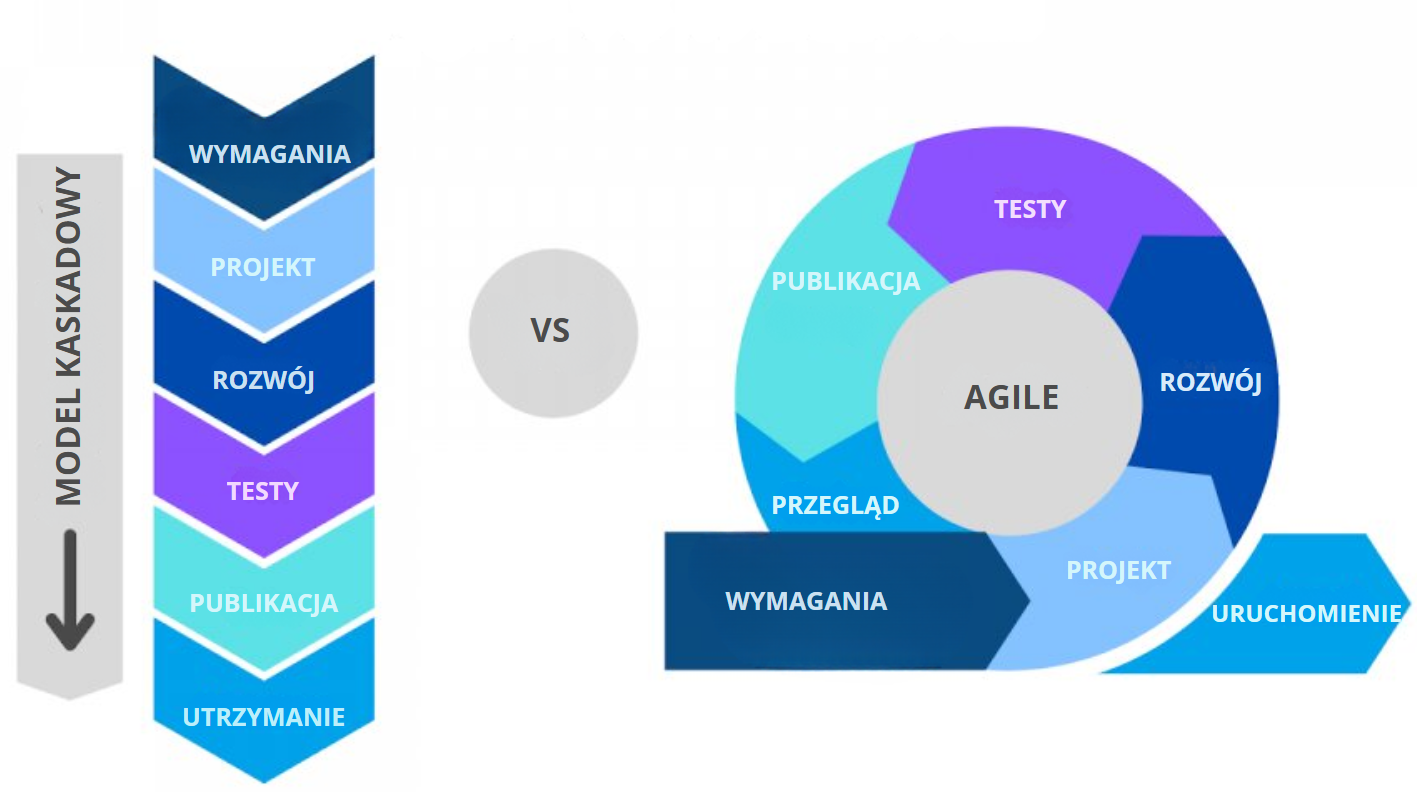
\includegraphics[width=1\linewidth]{img/waterfall_agile_PL.png}
    \caption*{Żródło: https://www.linkedin.com/pulse/waterfall-vs-agile-which-better-you-why-datacademy-cloud/}
\end{figure}

\subsection{Różnorodne technologie}
Różnorodność technologii w branży IT jest bardzo duża i kompetencje oraz wiedza specjalistów mogą się bardzo różnić pomiędzy zajmowanymi stanowiskami. 
Różnice te często znacznie utrudniają komunikację nawet wewnątrz zespołu projektowego. Na przykład:
\begin{itemize}
    \item Specjaliści od sprzętu mogą nie rozumieć języka analityków baz danych i odwrotnie.
    \item Eksperci ds. bezpieczeństwa mogą mieć trudności w dialogu z analitykami biznesowymi.
\end{itemize}

Nawet osoby pracujące w tej samej dziedzinie IT czasem się nie rozumieją, jeśli korzystają z innych technologii. Przykładowo, jeśli programista jest specjalistą w języku Java, to może mieć problem ze zrozumieniem pewnych zagadnień charakterystycznych dla języka Python, co ponownie może powodować zakłócenia w komunikacji.

Kolejnym wyzwaniem związanym z różnorodnością technologii jest ich szybka zmienność. Zespół może być bliski ukończenia projektu, gdy odkryje nowe rozwiązanie, które znacząco ulepszy produkt i lepiej zaspokoi długoterminowe potrzeby biznesowe. Nowe technologie skróciły też czas, jaki firmy mają na opracowanie, wdrożenie i dystrybucję produktów czy usług. To dynamiczne środowisko wymaga równie szybkich procesów zarządzania projektami IT. \autocite{ITPM}

\subsection{Specjaliści IT}
Inwestycje w technologie informatyczne są ściśle związane z rosnącym zapotrzebowaniem na wykwalifikowanych pracowników. Innymi słowy, jednym z głównych czynników sukcesu projektów IT są umiejętności techniczne zespołu. Według Tohidi specjaliści IT są zazwyczaj silni w dziedzinie podejmowania decyzji, jednak mają oni często duże braki komunikacyjne. Większość z nich jest introwertykami i brakuje im umiejętności, takich jak:
\begin{itemize}
    \item Umiejętności wsparcia: Przyjazne i taktowne podejście, cierpliwość, empatia wobec osób zestresowanych lub mających obawy, wysłuchiwanie skarg i problemów oraz uwzględnianie potrzeb innych.
    \item Szkolenie i doradztwo: Dostarczanie szkoleń i praktycznych porad, tworzenie kontekstu ułatwiającego rozwój umiejętności, wspieranie przedsiębiorczości i optymalizacja procesów biznesowych.
    \item Zarządzanie postawami i budowanie zespołu: Rozwiązywanie konfliktów, motywowanie do współpracy, identyfikowanie kluczowych obszarów biznesowych.
    \item Networking: Nieformalna komunikacja z osobami posiadającymi wartościowe informacje, utrzymywanie regularnych kontaktów (spotkania, rozmowy telefoniczne, korespondencja) oraz uczestnictwo w wydarzeniach społecznych.
\end{itemize}

Według badań komunikacja ma zaś bezpośrednie przełożenie na sukces projektu. \autocite{komunikacja} Nawet technicznie doskonałe inicjatywy często upadają z powodu jej braku. \autocite{Tohidi}

\subsection{Ryzyka w projektach IT}
Wszystkie projekty są ryzykowne, ponieważ stanowią unikalne przedsięwzięcia o różnym stopniu złożoności, których celem jest dostarczanie korzyści. Realizowane są one w kontekście ograniczeń i założeń, przy jednoczesnym uwzględnianiu oczekiwań interesariuszy, które mogą być sprzeczne i zmienne. Organizacje powinny podejmować ryzyko projektowe w sposób kontrolowany i świadomy, aby tworzyć wartość, równoważąc ryzyko i zysk. \autocite{pmbok6}

Niepewność to brak zrozumienia i świadomości w zakresie problemów, zdarzeń, ścieżek działania lub rozwiązań do wdrożenia. Ryzyko zaś jest aspektem niepewności. Ryzyko definiuje się jako niepewne zdarzenie lub warunek, które w przypadku wystąpienia może wywrzeć pozytywny lub negatywny wpływ na jeden lub więcej celów projektu. Ryzyka negatywne nazywane są zagrożeniami, zaś pozytywne – szansami. Wszystkie projekty obarczone są ryzykiem, ponieważ są to unikalne przedsięwzięcia charakteryzujące się różnym stopniem niepewności. \autocite{pmbok7}

Projekty informatyczne niosą za sobą pewne specyficzne dla nich aspekty ryzyka, takie jak skłonność inżynierów do dodawania niepotrzebnych funkcji (ang. feature creep) czy ryzyka związane z niematerialnym charakterem oprogramowania. Szczególną uwagę należy poświęcić ryzykom związanym z wymaganiami jakościowymi oprogramowania, takimi jak bezpieczeństwo funkcjonalne (ang. safety) czy bezpieczeństwo IT (ang. security). \autocite{program}\autocite{swebok}

Poniżej została przedstawiona przykładowa propozycja kwestionariusza ryzyk dla projektu informatycznego, ryzyka zostały podzielone na pięć kategorii: \autocite{ITPM}

\begin{itemize}
    \item Ryzyko rynkowe:
    \begin{itemize}
        \item Czy projekt IT, który ma stworzyć nowy produkt lub usługę, będzie przydatny dla organizacji lub nadający się do sprzedaży?
        \item Czy użytkownicy zaakceptują i będą korzystać z produktu/usługi?
        \item Czy konkurencja nie opracuje lepszego rozwiązania szybciej, czyniąc projekt stratą czasu i pieniędzy?
    \end{itemize} 
    \item Ryzyko finansowe:
    \begin{itemize}
        \item Czy organizacja może sobie pozwolić na realizację projektu?
        \item Jak bardzo interesariusze ufają prognozom finansowym?
        \item Czy projekt spełni szacunki dotyczące wartości bieżącej netto (NPV), zwrotu z inwestycji (ROI) i okresu zwrotu?
        \item Jeśli nie, czy organizacja będzie w stanie kontynuować projekt?
        \item Czy ten projekt to najlepsze wykorzystanie środków finansowych organizacji?
    \end{itemize} 
    \item Ryzyko technologiczne:
    \begin{itemize}
        \item Czy projekt jest wykonalny technicznie?
        \item Czy wykorzysta technologie dojrzałe, nowoczesne czy eksperymentalne?
        \item Kiedy zapadną decyzje dotyczące wyboru technologii?
        \item Czy sprzęt, oprogramowanie i sieci będą działać prawidłowo?
        \item Czy technologia będzie dostępna na czas, aby osiągnąć cele projektu?
        \item Czy technologia zdezaktualizuje się, zanim powstanie użyteczny produkt?
    \end{itemize}
    \item Ryzyko kadrowe:
    \begin{itemize}
        \item Czy organizacja ma pracowników z odpowiednimi kompetencjami, aby pomyślnie zrealizować projekt?
        \item Jeśli nie, czy można znaleźć takie osoby?
        \item Czy zespół posiada umiejętności menedżerskie i techniczne?
        \item Czy członkowie zespołu mają wystarczające doświadczenie?
        \item Czy kierownictwo wyższego szczebla wspiera projekt?
        \item Czy istnieje rzecznik projektu (ang. project champion)?
        \item Czy organizacja zna sponsora/klienta projektu?
        \item Jak dobra jest relacja ze sponsorem/klientem?
    \end{itemize}
    \item Ryzyko strukturalne/procesowe:
    \begin{itemize}
        \item Na jakim poziomie zmiany wprowadzi projekt w obszarach użytkowników i procedurach biznesowych?
        \item Ile różnych grup użytkowników musi zadowolić projekt?
        \item Z iloma innymi systemami musi współdziałać nowy projekt/system?
        \item Czy organizacja ma wypracowane procesy umożliwiające sukces projektu?
    \end{itemize}
\end{itemize}

\subsubsection{Czasowy model ryzyk}
Ciekawa interpretacja i zrozumienie ryzyk w projektach informatycznych zostało zawarte w pracy Gemino. \autocite{ryzyka} Zwraca on uwagę na czasowy charakter projektów (rozumiany jako przejście od warunków początkowych, przez przebieg projektu, aż do jego rezultatów). Dzięki czemu proponuje inną formę kategoryzacji ryzyk w projektach informatycznych, uwzględniającą różnice między ryzykami obecnymi w momencie definiowania projektu a tymi, które pojawiają się lub są ujawniane podczas jego realizacji.

\textbf{Ryzyka a priori}\\
Niektóre cechy projektu, takie jak budżet, czas trwania, złożoność techniczna, niepewność wymagań, brak doświadczenia zespołu oraz niewystarczająca wiedza sponsora projektu, mogą być oszacowane przed rozpoczęciem projektu. Są to ryzyka a priori. Można wyróżnić dwie kategorie ryzyk a priori:
\begin{itemize}
    \item Ryzyka związane z elementami strukturalnymi projektu (np. czas trwania, budżet, nakład pracy, złożoność techniczna)
    \item Ryzyka wynikające z wiedzy dostępnej dla zespołu (np. kompetencje kierownika projektu, sponsora, członków zespołu)
\end{itemize}

Elementy strukturalne, takie jak wielkość projektu i złożoność techniczna, są uznawane za istotne ryzyka. \autocite{mcfarlan}\autocite{zmud} Są one znane a przynajmniej potencjalnie możliwe do określenia na początku projektu. Zarządzanie nimi wymaga stosowania tradycyjnych ("twardych") technik zarządzania projektami, takich jak podział pracy, estymacja, harmonogramowanie oraz budżetowanie.

Brak zasobów wiedzy (np. niedoświadczony kierownik projektu lub zespół) jest również ważną kategorią ryzyk w projektach informatycznych. \autocite{mcfarlan}\autocite{barki} Ryzyka te wymagają zastosowania technik zarządzania, które często określa się mianem „umiejętności miękkich”, takich jak komunikacja, budowanie zespołu, uczenie się i koordynacja wiedzy. 

\textbf{Ryzyka wyłaniające się}\\
Zanim projekt się rozpocznie, kierownik projektu wyrabia sobie oczekiwania co do poziomu wsparcia ze strony najwyższego kierownictwa oraz użytkowników. Jednakże oczekiwany poziom wsparcia lub uczestnictwa nie wpływa bezpośrednio na wyniki projektu. To właśnie rzeczywisty poziom wsparcia, ujawniony przez zachowania najwyższego kierownictwa i użytkowników, ma najbardziej bezpośredni wpływ na efektywność. \autocite{chaos} Na przykład, choć kierownik projektu może wierzyć, że otrzyma wysoki poziom uczestnictwa użytkowników, to rzeczywisty poziom uczestnictwa ujawnia się dopiero poprzez zachowania użytkowników w trakcie realizacji projektu. Kierownik wyższego szczebla może obiecywać wysoki poziom wsparcia, ale nie dostarczyć go w praktyce. Dlatego te ryzyka można określić jako ryzyka wyłaniające się (ang. Emergent Risks).

Można wyróżnić dwie kategorie ryzyk wyłaniających się:
\begin{itemize}
    \item Ryzyka związane z niedoborami wsparcia organizacyjnego (np. brak wsparcia sponsora, klienta lub użytkownika)
    \item Ryzyka związane ze zmianami, które zachodzą (np. zmiany celów, członków zespołu oraz szerszego otoczenia)
\end{itemize} \autocite{ryzyka}

Pierwszą z tych kategorii to ryzyko wsparcia organizacyjnego. Istnieją trzy kluczowe obszary wsparcia organizacyjnego — wsparcie sponsora wykonawczego, zaangażowanie menedżera klienta oraz uczestnictwo użytkowników. Wsparcie organizacyjne jest uznawane za kluczowe dla sukcesu projektu. Gdy poziom wsparcia organizacyjnego jest niższy niż oczekiwano, określa się to jako ryzyko (np. brak wsparcia ze strony kierownictwa). Natomiast gdy wsparcie organizacyjne spełnia lub przewyższa oczekiwania, traktuje się je jako istotny zasób dla kierowników projektów. \autocite{keil}\autocite{sharma}\autocite{yetton}

Drugą kategorię ryzyk stanowią zmiany wpływające na projekty, w tym zmiany celów projektu, kluczowych osób oraz warunków zewnętrznych, z którymi projekt musi się mierzyć. Są to ryzyka zmienności projektu. \autocite{gemino} Kategoria ta jest podobna do kategorii ryzyka „środowiskowego” zidentyfikowanej przez Keil. \autocite{keil} Ta zmienność często pozostaje poza kontrolą członków zespołu projektowego, ale może mieć znaczący wpływ na wyniki projektu. \autocite{ryzyka}

Omówione kategorie ryzyk zostały przedstawione w tabelach 4.1. oraz 4.2.

\begin{table}
    \caption{Kategoryzacja ryzyk według modelu czasowego}
    \centering
    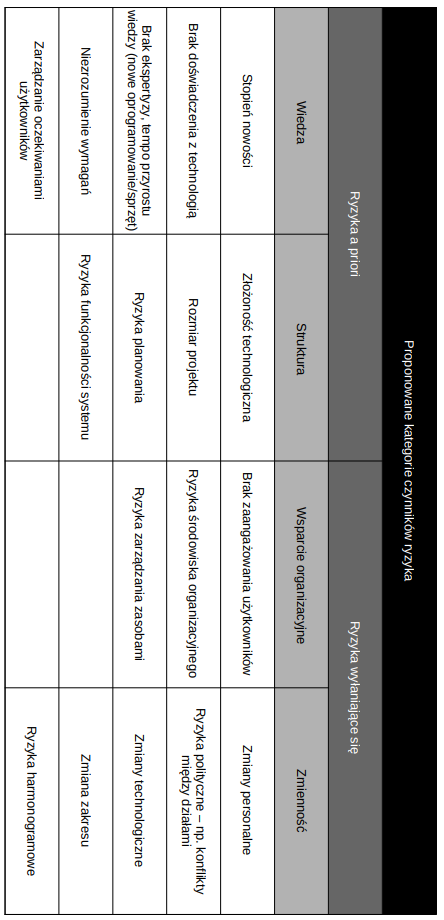
\includegraphics[width=0.5\linewidth]{img/ryzyka3.png}
    \caption*{Źródło: Gemino, Reich i Sauer, „A Temporal Model of Information Technology Project Performance” }
  \end{table}

\subsection{Ewaluacja projektów informatycznych}
Szybkie tempo zmian w technologii IT powoduje poważne trudności już na etapie rozpoczynania każdej dużej inwestycji. Każdy długoterminowy, sztywny projekt staje się niemal przestarzały, zanim w ogóle się rozpocznie, a w momencie pełnej instalacji jest już z pewnością nieaktualny. Nie oznacza to jednak, że nie należy dokonywać oceny projektów. Ocenianie lub uzasadnianie inwestycji w technologię informacyjną jest problematyczne. Inwestycje w technologię informacyjną są trudniejsze niż wiele innych decyzji inwestycyjnych, ponieważ koszty i korzyści trudno jest zidentyfikować i zmierzyć, a występujące czynniki niematerialne mogą mieć istotne znaczenie. \autocite{powell1992information}

Czasami wartość projektu informatycznego nie jest od razu znana w momencie wdrożenia systemu. Na przykład, celem projektu mającego na celu stworzenie witryny e-commerce powinno być generowanie zysków – a nie budowanie lub instalacja sprzętu, oprogramowania i stron internetowych na określonej platformie serwerowej. Technologia i jej późniejsze wdrożenie są jedynie środkiem do osiągnięcia celu. W związku z tym celem witryny e-commerce może być wygenerowanie 250 000 dolarów w ciągu sześciu miesięcy. W rezultacie ocena, czy projekt osiągnął swój cel, może nastąpić dopiero po wdrożeniu systemu. \autocite{ITPMMarchewka}

Komitety oceniające w organizacjach często stają przed wyborem, w którym konkurencyjne technologie nie dają się łatwo ze sobą porównać. Wynika to z faktu, że dwa projekty mogą zaspokajać różne, a nawet konkurencyjne wymagania. Ostateczna pozycja w rankingu technologii zależy od tego, w jakim stopniu każda z nich odpowiada na poszczególne wymagania. Jednak poza przypadkami, w których jedna technologia wyraźnie dominuje pozostałe, pojawia się problem, gdy dwie alternatywy zaspokajają odmienne i konkurencyjne potrzeby. Rozwiązanie takich konfliktów jest praktycznie niemożliwe bez udziału wiedzy eksperckiej w procesie podejmowania decyzji. \autocite{thomaidis2006evaluation}

Currie określa jednak uzasadnianie inwestycji w IT jako „rytuał legitymizacji”, a nie proces rzeczywistej oceny korzyści. \autocite{Currie1989} Jak zauważył Williams już pół wieku temu: „W biznesie nie chodzi o to, by tworzyć dobre prognozy, lecz by sprawiać, aby się one spełniały”. \autocite{williams1967technology}

\subsection{Ostatnie trendy w projektach informatycznych}
Ostatnie trendy, takie jak rosnąca globalizacja, outsourcing oraz zespoły wirtualne, stwarzają nowe wyzwania i możliwości dla kierowników projektów informatycznych oraz ich zespołów. \autocite{ITPM}

\subsubsection{Globalizacja}
Globalizacja to termin powszechnie używany, lecz o niejasnym znaczeniu, nawet wśród tych, którzy się nim posługują. \autocite{robertson2007globalization} Anthony McGrew twierdzi, że globalizacja stanowi sieć powiązań i połączeń wykraczających poza państwa narodowe (a tym samym społeczeństwa), które tworzą współczesny system światowy. To proces, w ramach którego wydarzenia, decyzje i działania w jednej części świata mogą mieć znaczące konsekwencje dla jednostek i społeczności w odległych regionach globu. \autocite{McGrew1990}

Globalizacja znacząco wpłynęła na sektor IT. Mimo że główne firmy technologiczne, takie jak Microsoft czy IBM, powstały w Stanach Zjednoczonych, większość ich działalności ma charakter globalny – przedsiębiorstwa i osoby z całego świata przyczyniają się do rozwoju technologii informacyjnych oraz współpracują przy różnych projektach IT. \autocite{ITPM}

Ma to również znaczący wpływ na pracę kierowników projektów, gdyż muszą oni uwzględnić następujące zagadnienia:

\begin{itemize}
  \item \textbf{Komunikacja}:  
  Praca w różnych strefach czasowych, różne języki, pochodzenie kulturowe i święta wymagają efektywnego planowania komunikacji.
  \item \textbf{Zaufanie}:  
  Zaufanie jest kluczowe dla wszystkich zespołów, zwłaszcza globalnych. Należy je budować od początku, szanując różnice i doceniając wartości, jakie członkowie wnoszą do projektu.
  \item \textbf{Wspólne praktyki pracy}:  
  Należy ujednolicić procesy pracy i wypracować praktyki akceptowane przez wszystkich. \autocite{ITPM}
\end{itemize}

\subsubsection{Outsourcing}
Outsourcing oznacza pozyskiwanie dóbr i usług przez organizację z zewnętrznych źródeł. Termin offshoring odnosi się do outsourcingu realizowanego w innym kraju. Offshoring jest naturalną konsekwencją globalizacji. Projekty IT coraz częściej opierają się na outsourcingu, zarówno w granicach kraju, jak i poza nimi. Niektóre organizacje utrzymują konkurencyjność, strategicznie wykorzystując outsourcing. Wielu firmom udało się obniżyć koszty dzięki tej praktyce, mimo że bywa ona niepopularna w ich krajach macierzystych. \autocite{ITPM} Słynnym przykładem outsourcingu jest decyzja Eastmana Kodaka o przekazaniu całego centrum danych firmie IBM, operacji mikrokomputerowych Businessland oraz sieci telekomunikacyjnych i danych Digital Equipment Corporation oraz IBM.

Outsourcing IT zależy od wielu czynników na różnych poziomach. Na poziomie gospodarczym trendy i cykle ekonomiczne mogą motywować firmy do racjonalizacji zarządzania infrastrukturą IT poprzez outsourcing. Na poziomie branżowym presja konkurencyjna skłania firmy do budowania „partnerskich relacji” z kluczowymi dostawcami IT. Na poziomie firmy poszukiwanie przewagi konkurencyjnej jest kluczowym impulsem do decyzji o outsourcingu. Wewnątrz firmy decyzja o outsourcingu może zależeć od czynników menedżerskich, takich jak dążenie do kontroli zasobów lub postrzeganie informacji jako źródła władzy. \autocite{loh1992determinants}\autocite{Kanter1979}\autocite{Mintzberg1983}

W związku z rosnącym wykorzystaniem outsourcingu w projektach IT, kierownicy projektów muszą lepiej zrozumieć globalne i zamówieniowe aspekty, w tym pracę z zespołami zdalnymi. \autocite{ITPM}  

\subsubsection{Zespoły zdalne}
Globalizacja projektów zwiększyła zapotrzebowanie na zespoły zdalne, \autocite{pmbok6} czyli grupy osób współpracujących pomimo granic czasowych i przestrzennych, wykorzystujące technologie komunikacyjne. Członkowie zespołu mogą pracować dla tej samej firmy w jednym kraju lub obejmować pracowników, niezależnych konsultantów, dostawców, a nawet wolontariuszy z całego świata. \autocite{ITPM}

W konkurencyjnym rynku zespoły zdalne stanowią coraz częstsze rozwiązanie odpowiadające na potrzebę skrócenia czasu wprowadzenia produktu na rynek, obniżenia kosztów oraz szybkiego rozwiązywania złożonych problemów organizacyjnych. Zespoły wirtualne umożliwiają organizacjom łączenie talentów i ekspertyzy pracowników oraz osób z zewnątrz poprzez eliminację barier czasowych i przestrzennych. Obecnie firmy intensywnie inwestują w zespoły zdalne, aby podnieść swoją wydajność i konkurencyjność. \autocite{ebrahim2009virtual}

\textbf{Zalety zespołów wirtualnych}  
\begin{itemize}
  \item \textbf{Obniżenie kosztów} – wielu pracowników zdalnych nie wymaga biur ani dodatkowego wsparcia.
  \item \textbf{Dostęp do ekspertyzy i elastyczność} – globalny zasięg umożliwia pracę przez całą dobę, zwiększając konkurencyjność.
  \item \textbf{Lepsza równowaga praca–życie} – brak sztywnych godzin pracy i dojazdów.
\end{itemize}

\textbf{Wady zespołów wirtualnych}  
\begin{itemize}
  \item \textbf{Izolacja członków} – trudności w adaptacji do środowiska zdalnego.
  \item \textbf{Problemy komunikacyjne} – brak języka ciała i komunikacji niewerbalnej utrudnia budowanie relacji.
  \item \textbf{Ograniczenie nieformalnej wymiany informacji} – trudności w nawiązywaniu kontaktów.
  \item \textbf{Zależność od technologii} – awarie mogą sparaliżować pracę.
\end{itemize}


